\documentclass[
  xcolor={svgnames},
  hyperref={colorlinks,citecolor=DeepPink4,linkcolor=DarkRed,urlcolor=DarkBlue}
  ]{beamer}
\usepackage{amsmath}
\usepackage{amssymb}
\usepackage{amsfonts}
\usepackage[utf8]{inputenc}
\usepackage{graphicx}
\usepackage{hyperref}
\usepackage{xcolor}
\usepackage{wasysym}
\usepackage{listings}
\usepackage{tikz}
\usepackage[normalem]{ulem}
\usepackage{textcomp}
\usepackage{verbatim}
\usepackage[T1]{fontenc}
\usepackage{lmodern}
\usepackage[framemethod=tikz]{mdframed}
\usetikzlibrary{shapes.callouts,shadows, calc}

\tikzset{note/.style={rectangle callout, rounded corners,fill=gray!20,drop shadow,font=\footnotesize}}    
\newcommand{\tikzmark}[1]{\tikz[overlay,remember picture] \node (#1) {};}    

\newcounter{image}
\setcounter{image}{1}

\makeatletter
\newenvironment{btHighlight}[1][]
{\begingroup\tikzset{bt@Highlight@par/.style={#1}}\begin{lrbox}{\@tempboxa}}
{\end{lrbox}\bt@HL@box[bt@Highlight@par]{\@tempboxa}\endgroup}

\newcommand\btHL[1][]{%
  \begin{btHighlight}[#1]\bgroup\aftergroup\bt@HL@endenv%
}
\def\bt@HL@endenv{%
  \end{btHighlight}%   
  \egroup
}
\newcommand{\bt@HL@box}[2][]{%
  \tikz[#1]{%
    \pgfpathrectangle{\pgfpoint{0pt}{0pt}}{\pgfpoint{\wd #2}{\ht #2}}%
    \pgfusepath{use as bounding box}%
    \node[anchor=base west,rounded corners, fill=green!30,outer sep=0pt,inner xsep=0.2em, inner ysep=0.1em,  #1](a\theimage){\usebox{#2}};
  }%
 \stepcounter{image}
}
\makeatother

\usetheme{Warsaw}
\usecolortheme{lily}
\setbeamercovered{transparent}
\setbeamertemplate{headline}{
  \begin{beamercolorbox}{section in head/foot}
    \vskip2pt\insertnavigation{\paperwidth}\vskip2pt
  \end{beamercolorbox}
}

\setbeamertemplate{footline}{
}

\author{
  {\tiny Tony Morris\\}
}

\xdefinecolor{darkgreen}{rgb}{0,0.35,0}
\lstset{
  tabsize=2,
  basicstyle=\ttfamily,
  moredelim=**[is][\btHL]{`}{`}
}
\lstdefinelanguage{java}{
  morekeywords={abstract,assert,boolean,break%
    byte,case,catch,char,class,const,continue%
    default,do,double,else,enum,extends,false%
    final,finally,float,for,goto,if,implements%
    import,instanceof,int,interface,long,native%
    new,null,package,private,protected,public%
    return,short,static,strictfp,super,switch%
    synchronized,this,throw,throws,transient%
    true,try,void,volatile,while},
  otherkeywords={=,=>,<-,<\%,<:,>:,\#,@},
  sensitive=true,
  morecomment=[l]{//},
  morecomment=[n]{/*}{*/},
  morestring=[b]",
  morestring=[b]',
  morestring=[b]"""
}
\lstdefinelanguage{csharp}
{
  sensitive=true,
  morekeywords=[1]{
  abstract, as, base, break, case,
  catch, checked, class, const, continue,
  default, delegate, do, else, enum,
  event, explicit, extern, false,
  finally, fixed, for, foreach, goto, if,
  implicit, in, interface, internal, is,
  lock, namespace, new, null, operator,
  out, override, params, private,
  protected, public, readonly, ref,
  return, sealed, sizeof, stackalloc,
  static, struct, switch, this, throw,
  true, try, typeof, unchecked, unsafe,
  using, virtual, volatile, while, bool,
  byte, char, decimal, double, float,
  int, lock, object, sbyte, short, string,
  uint, ulong, ushort, void},
  morecomment=[l]{//},
  morecomment=[s]{/*}{*/},
  morecomment=[l][keywordstyle4]{\#},
  morestring=[b]",
  morestring=[b]',
}
\lstdefinelanguage{haskell}{
  morekeywords={class,instance,where,do,data,newtype,default,deriving,module},
  otherkeywords={<-},
  sensitive=true,
  morecomment=[l]{--},
  morecomment=[n]{\{-}{-\}}, 
  morestring=[b]",
  morestring=[b]',
  morestring=[b]"""
}
\lstdefinelanguage{python}{
 keywords={catch, def, float, lambda, in, int, null, self, str, switch, typeof},
 keywordstyle=\color{ForestGreen}\bfseries,
 ndkeywords={boolean, throw, import},
 ndkeywords={return, class, if ,elif, endif, while, do, else, True, False , catch, def},
 ndkeywordstyle=\color{red}\bfseries,
 identifierstyle=\color{black},
 sensitive=false,
 comment=[l]{\#},
 morecomment=[s]{/*}{*/},
 commentstyle=\color{purple}\ttfamily,
 stringstyle=\color{red}\ttfamily,
}
\lstdefinelanguage{scala}{
  morekeywords={abstract,case,catch,class,def,%
    do,else,extends,false,final,finally,%
    for,forSome,if,implicit,import,lazy,match,%
    new,null,object,override,package,%
    private,protected,requires,return,sealed,%
    super,this,throw,trait,true,try,%
    type,val,var,while,with,yield},
  otherkeywords={=,=>,<-,<\%,<:,>:,\#,@},
  sensitive=true,
  morecomment=[l]{//},
  morecomment=[n]{/*}{*/},
  morestring=[b]",
  morestring=[b]',
  morestring=[b]"""
}
\lstdefinestyle{haskell}{
  language=haskell,
  basicstyle=\footnotesize\ttfamily,
  stringstyle=\color{darkgreen}\ttfamily,
  commentstyle=\color{gray}\ttfamily,
  keywordstyle=\footnotesize\color{blue}\ttfamily,
  tabsize=2,
  moredelim=**[is][\btHL]{`}{`}
}
\lstdefinestyle{java}{
  language=java,
  basicstyle=\footnotesize\ttfamily,
  stringstyle=\color{darkgreen}\ttfamily,
  commentstyle=\color{gray}\ttfamily,
  keywordstyle=\footnotesize\color{blue}\ttfamily,
  tabsize=2,
  moredelim=**[is][\btHL]{`}{`}
}
\lstdefinestyle{python}{
  language=python,
  basicstyle=\footnotesize\ttfamily,
  stringstyle=\color{darkgreen}\ttfamily,
  commentstyle=\color{gray}\ttfamily,
  keywordstyle=\footnotesize\color{blue}\ttfamily,
  tabsize=2,
  moredelim=**[is][\btHL]{`}{`}
}
\lstdefinestyle{csharp}{
  language=csharp,
  basicstyle=\tiny\ttfamily,
  stringstyle=\color{darkgreen}\ttfamily,
  commentstyle=\color{gray}\ttfamily,
  keywordstyle=\tiny\color{blue}\ttfamily,
  tabsize=2,
  moredelim=**[is][\btHL]{`}{`}
}
\lstdefinestyle{scala}{
  language=scala,
  basicstyle=\footnotesize\ttfamily,
  stringstyle=\color{darkgreen}\ttfamily,
  commentstyle=\color{gray}\ttfamily,
  keywordstyle=\footnotesize\color{blue}\ttfamily,
  tabsize=2,
  moredelim=**[is][\btHL]{`}{`}
}
% #866eaa
\definecolor{nicta-purple}{rgb}{0.5234,0.4297,0.6640}

\defbeamertemplate*{title page}{customized}[1][] {
  \centering
  \color{nicta-purple}
  \usebeamerfont{title}\inserttitle\par
  \bigskip
  \usebeamerfont{subtitle}\insertsubtitle\par
  \bigskip
  \bigskip
  \bigskip
  \bigskip
  \usebeamerfont{institute}\insertinstitute\par
  \bigskip
  \usebeamerfont{author}\insertauthor\par
  % \usebeamerfont{date}\insertdate\par
  \usebeamercolor[fg]{titlegraphic}\inserttitlegraphic
}

\logo{
\includegraphics[height=0.8cm]{image/data61-csiro.jpg}}


\setbeamercovered{transparent}

\begin{document}

\newmdenv[tikzsetting={draw=black,fill=white,fill opacity=0.7, line width=4pt},backgroundcolor=none,leftmargin=0,rightmargin=0,innertopmargin=4pt]{Conference}

\newmdenv[tikzsetting={draw=black,fill=white,fill opacity=0.7, line width=4pt},backgroundcolor=none,leftmargin=0,rightmargin=0,innertopmargin=4pt,skipbelow=\baselineskip,%
skipabove=\baselineskip]{TitleBox}

\title{\large List Folds}
\institute[Data61]{Data61, CSIRO}

{
  \usebackgroundtemplate{
\includegraphics[width=1.0\paperwidth]{image/title-background.png}}

  \begin{frame}[plain] 

  \begin{TitleBox}
    \begin{center}
    {\huge \inserttitle}

    \hspace{1em}
    
    {\huge \insertsubtitle}
    \end{center}
  \end{TitleBox}

  \vspace{3em}

  \begin{Conference}
    \begin{center}
    \tiny{Brisbane Functional Programming Group, November 2016}

    \hspace{1em}

    {\insertauthor}
    \end{center}
  \end{Conference}

  \end{frame}
}

\begin{frame}
\frametitle{Intro}
\begin{block}{Explain List Folds to Yourself, April 2013}
In April 2013, BFPG had a chat about list folds
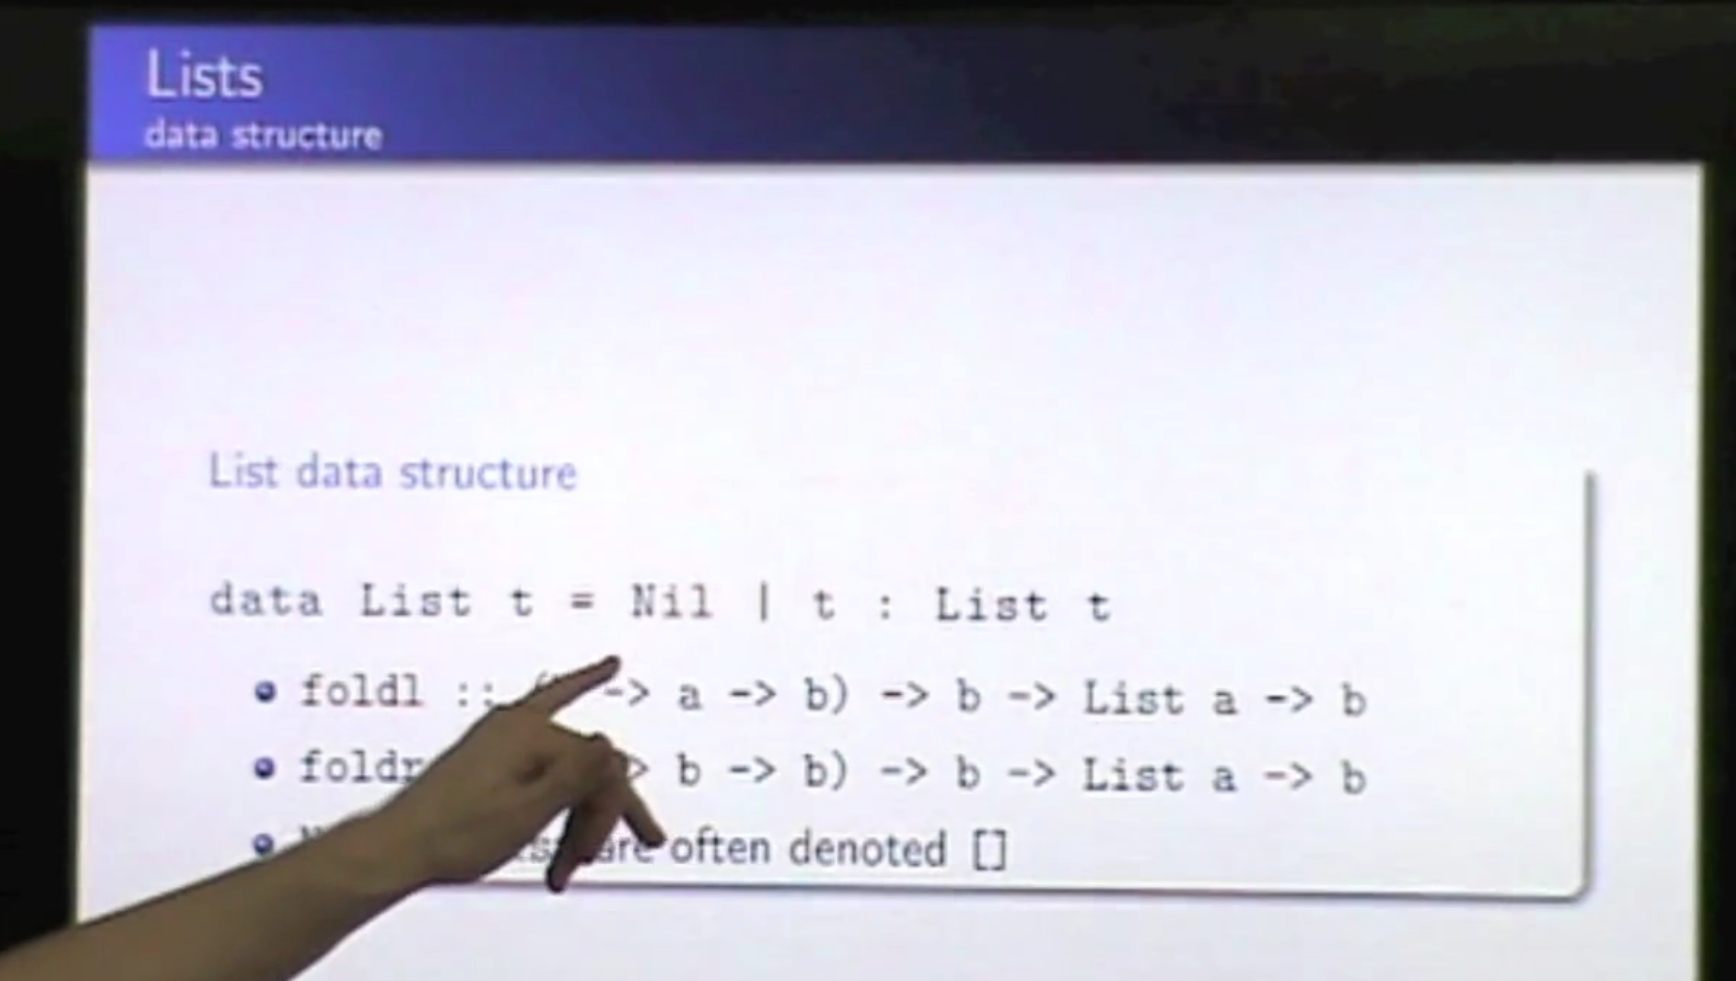
\includegraphics[height=0.5\textheight]{image/list-folds-2013.png}
\end{block}
\end{frame}

\begin{frame}
\frametitle{Introduction}
\begin{block}{Today}
\begin{itemize}
\item<1-> we are doing a similar thing, with differences
\item<2-> aiming to beginners, who have only had cursory experiences with lists
\item<3-> being very explicit about the utility of the developed intuition, and developing it further
\item<4-> interactive exercises and puzzles with the newly-developed intuition (be brave!)
\end{itemize}
\end{block}
\end{frame}

\begin{frame}
\frametitle{Lists}
\begin{block}{What is a list?}
What, exactly is a list?
\end{block}
\end{frame}

\begin{frame}
\frametitle{Lists}
\begin{block}{a list is either}
\begin{itemize}
\item a \textbf{Nil} construction, with no associated data
\item a \textbf{Cons} construction, associated with one arbitrary value, and another list
\end{itemize}
\end{block}
\emph{And \textbf{never, ever} anything else}
\end{frame}

\begin{frame}[fragile]
\frametitle{Lists}
\begin{block}{a list using C\#}
\begin{lstlisting}[style=csharp,basicstyle=\scriptsize\ttfamily,mathescape]
interface List<A>{}
class Nil<A> : List<A> {}
class Cons<A> : List<A> { A head; List<A> tail; }
\end{lstlisting}
\end{block}
\tiny{\emph{And some tricks to enforce \textbf{never ever anything else}}}
\end{frame}

\begin{frame}[fragile]
\frametitle{Lists}
\begin{block}{a list using Haskell}
\begin{lstlisting}[style=haskell,basicstyle=\scriptsize\ttfamily,mathescape]
data List a = Nil | Cons a (List a)
\end{lstlisting}
\end{block}
\tiny{\emph{\textbf{never ever anything else} is enforced in haskell}}
\end{frame}

\begin{frame}[fragile]
\frametitle{Some examples of Lists}
\begin{block}{C\#}
\begin{lstlisting}[style=csharp,basicstyle=\scriptsize\ttfamily,mathescape]
new Cons<int>(12, new Nil<int>())
\end{lstlisting}
\end{block}
\begin{block}{Haskell}
\begin{lstlisting}[style=haskell,basicstyle=\scriptsize\ttfamily,mathescape]
Cons 12 Nil
\end{lstlisting}
\end{block}
\end{frame}

\begin{frame}[fragile]
\frametitle{Some examples of Lists}
\begin{block}{C\#}
\begin{lstlisting}[style=csharp,basicstyle=\tiny\ttfamily,mathescape]
new Cons<char>('a', new Cons<char>('b', new Cons<char>('c', new Nil<char>())))
\end{lstlisting}
\end{block}
\begin{block}{Haskell}
\begin{lstlisting}[style=haskell,basicstyle=\scriptsize\ttfamily,mathescape]
Cons 'a' (Cons 'b' (Cons 'c' Nil))
\end{lstlisting}
\end{block}
\end{frame}

\begin{frame}
\frametitle{Some nomenclature}
\begin{block}{Naming Schmaming}
\begin{itemize}
\item<1-> Sometimes you will see \lstinline{Nil} denoted \lstinline{[]}
\item<2-> and/or \lstinline{Cons} denoted \lstinline{:} in an infix position
\item<3-> like this \lstinline{1:(2:(3:[]))}
\item<4-> but this is the same data structure
\end{itemize}
\end{block}
\end{frame}

\begin{frame}
\frametitle{Lists}
\begin{center}
Ensure we all know what a list is
\end{center}
\end{frame}

\begin{frame}
\frametitle{Folds}

TODO

\end{frame}



\begin{frame}
\frametitle{foldl}
The \lstinline[basicstyle=\ttfamily]$foldl$ function accepts three values:
\begin{enumerate}
\item \lstinline[basicstyle=\ttfamily]$f :: b -> a -> b$
\item \lstinline[basicstyle=\ttfamily]$z :: b$
\item \lstinline[basicstyle=\ttfamily]$list :: List a$
\end{enumerate}
to get back a value of the type \lstinline[basicstyle=\ttfamily]$b$.

\hrulefill

\lstinline[basicstyle=\ttfamily]$foldl :: (b -> a -> b) -> b -> List a -> b$
\lstinline[basicstyle=\ttfamily]$B foldLeft<A, B>(Func<B, A, B>, B, List<A>)$
\end{frame}

\begin{frame}
\frametitle{foldl}
\begin{block}{?}
\begin{center}
How does \lstinline[basicstyle=\ttfamily]$foldl$ take three values to that return value?
\end{center}
\end{block}
\end{frame}

\begin{frame}[fragile]
\frametitle{foldl}
\begin{block}{all left folds are loops}
\begin{lstlisting}[style=haskell,basicstyle=\scriptsize\ttfamily,mathescape]
\f z list ->
  var r = z
  foreach(a in list)
    r = f(r, a)
  return r
\end{lstlisting}
\end{block}
\end{frame}

\begin{frame}[fragile]
\frametitle{foldl}
\begin{block}{all left folds are loops}
\begin{lstlisting}[style=haskell,basicstyle=\scriptsize\ttfamily,mathescape]
\f z list ->
  var r = `z`
  foreach(a in `list`)
    r = `f`(r, a)
  return r
\end{lstlisting}
\end{block}
\end{frame}

\begin{frame}[fragile]
\frametitle{foldl}
\begin{block}{all left folds are loops}
Let's sum the integers of a list
\end{block}
\end{frame}

\begin{frame}[fragile]
\frametitle{foldl}
\begin{block}{sum the integers of a list}
\begin{lstlisting}[style=haskell,basicstyle=\scriptsize\ttfamily,mathescape]
\f z list ->
  var r = `z`
  foreach(a in `list`)
    r = `f`(r, a)
  return r
\end{lstlisting}
\end{block}
\begin{center}
\LARGE
?
\end{center}
\end{frame}

\begin{frame}[fragile]
\frametitle{foldl}
\begin{block}{sum the integers of a list}
\begin{lstlisting}[style=haskell,basicstyle=\scriptsize\ttfamily,mathescape]
\list ->
  var r = `0`
  foreach(a in `list`)
    r = `+`(r, a)
  return r
\end{lstlisting}
\end{block}
\end{frame}

\begin{frame}[fragile]
\frametitle{foldl}
\begin{block}{sum the integers of a list}
\begin{lstlisting}[style=haskell,basicstyle=\scriptsize\ttfamily,mathescape]
sum list = foldl (\r a -> (+) r a) 0 list
sum = foldl (+) 0
\end{lstlisting}
\end{block}
\end{frame}

\begin{frame}[fragile]
\frametitle{foldl}
\begin{block}{all left folds are loops}
Let's reverse a list
\end{block}
\end{frame}

\begin{frame}[fragile]
\frametitle{foldl}
\begin{block}{reverse a list}
\begin{lstlisting}[style=haskell,basicstyle=\scriptsize\ttfamily,mathescape]
\f z list ->
  var r = `z`
  foreach(a in `list`)
    r = `f`(r, a)
  return r
\end{lstlisting}
\end{block}
\begin{center}
\LARGE
?
\end{center}
\end{frame}

\begin{frame}[fragile]
\frametitle{foldl}
\begin{block}{reverse a list}
\begin{lstlisting}[style=haskell,basicstyle=\scriptsize\ttfamily,mathescape]
flipCons r a = Cons a r

\list ->
  var r = `Nil`
  foreach(a in `list`)
    r = `flipCons`(r, a)
  return r
\end{lstlisting}
\end{block}
\end{frame}

\begin{frame}[fragile]
\frametitle{foldl}
\begin{block}{reverse a list}
\begin{lstlisting}[style=haskell,basicstyle=\scriptsize\ttfamily,mathescape]
reverse list = foldl (\r a -> Cons a r) Nil list
reverse = foldl (flip Cons) Nil
\end{lstlisting}
\end{block}
\end{frame}

\begin{frame}[fragile]
\frametitle{foldl}
\begin{block}{all left folds are loops}
Let's compute the length of a list
\end{block}
\end{frame}

\begin{frame}[fragile]
\frametitle{foldl}
\begin{block}{length of a list}
\begin{lstlisting}[style=haskell,basicstyle=\scriptsize\ttfamily,mathescape]
\f z list ->
  var r = `z`
  foreach(a in `list`)
    r = `f`(r, a)
  return r
\end{lstlisting}
\end{block}
\begin{center}
\LARGE
?
\end{center}
\end{frame}

\begin{frame}[fragile]
\frametitle{foldl}
\begin{block}{length of a list}
\begin{lstlisting}[style=haskell,basicstyle=\scriptsize\ttfamily,mathescape]
plus1 r a = r + 1

\list ->
  var r = `0`
  foreach(a in `list`)
    r = `plus1`(r, a)
  return r
\end{lstlisting}
\end{block}
\end{frame}

\begin{frame}[fragile]
\frametitle{foldl}
\begin{block}{length of a list}
\begin{lstlisting}[style=haskell,basicstyle=\scriptsize\ttfamily,mathescape]
length list = foldl (\r a -> r + 1) 0 list
length = foldl (const . (+1)) 0
\end{lstlisting}
\end{block}
\end{frame}

\begin{frame}
\frametitle{foldl}
\begin{block}{refactoring, intuition}
\begin{itemize}
\item<1-> a left fold is what you would write if I insisted you remove all duplication from your loops
\item<2-> all left folds are exactly this loop
\item<3-> \textbf{exactly}
\end{itemize}
\end{block}
\end{frame}

\begin{frame}
\frametitle{foldl}
\begin{block}{some observations}
\begin{itemize}
\item<1-> a left fold will \textbf{never} work on an infinite list
\item<2-> a correct intuition for left folds is easy to build on existing programming knowledge (loop)
\end{itemize}
\end{block}
\end{frame}

\begin{frame}
\frametitle{Lists}
\begin{center}
Ensure we have developed intuition for left fold
\end{center}
\end{frame}

\begin{frame}
\frametitle{foldl}
The \lstinline[basicstyle=\ttfamily]$foldr$ function accepts three values:
\begin{enumerate}
\item \lstinline[basicstyle=\ttfamily]$f :: a -> b -> b$
\item \lstinline[basicstyle=\ttfamily]$z :: b$
\item \lstinline[basicstyle=\ttfamily]$list :: List a$
\end{enumerate}
to get back a value of the type \lstinline[basicstyle=\ttfamily]$b$.

\hrulefill

\lstinline[basicstyle=\ttfamily]$foldr :: (a -> b -> b) -> b -> List a -> b$
\lstinline[basicstyle=\ttfamily]$B FoldRight<A, B>(Func<A, B, B>, B, List<A>)$
\end{frame}

\begin{frame}
\frametitle{foldl}
\begin{block}{?}
\begin{center}
How does \lstinline[basicstyle=\ttfamily]$foldr$ take three values to that return value?
\end{center}
\end{block}
\end{frame}

\begin{frame}
\frametitle{foldr}
\begin{block}{constructor replacement}
The \lstinline[basicstyle=\ttfamily]$foldr$ function performs \textbf{constructor replacement}.
\end{block}
The expression \lstinline[basicstyle=\ttfamily]$foldr f z list$ replaces in \lstinline[basicstyle=\ttfamily]$list$:
\begin{itemize}
\item Every occurrence of \lstinline{Cons} \lstinline[basicstyle=\ttfamily]$(:)$ with \lstinline[basicstyle=\ttfamily]$f$.
\item Any occurrence of \lstinline{Nil} \lstinline[basicstyle=\ttfamily]$[]$ with \lstinline[basicstyle=\ttfamily]$z$\footnote{The \lstinline{Nil} constructor may be absent \textemdash an infinite list}.
\end{itemize}
\end{frame}

\begin{frame}
\frametitle{foldr}
\begin{block}{constructor replacement?}
\small
\begin{itemize}
\item suppose \lstinline[basicstyle=\ttfamily]$list = Cons A (Cons B (Cons C (Cons D Nil)))$
\item the expression \lstinline[basicstyle=\ttfamily, mathescape]!foldr f z list!
\item produces \lstinline[basicstyle=\ttfamily]$f A (f B (f C (f D z)))$
\end{itemize}
\end{block}
\end{frame}

\begin{frame}[fragile]
\frametitle{foldr}
\begin{block}{right folds replace constructors}
Let's multiply the integers of a list
\end{block}
\end{frame}

\begin{frame}[fragile]
\frametitle{foldr}
\begin{block}{multiply the integers of a list}
Supposing 
\begin{lstlisting}[style=haskell,basicstyle=\scriptsize\ttfamily,mathescape]
list = Cons 4 (Cons 5 (Cons 6 (Cons 7 Nil)))
\end{lstlisting}
\end{block}
\end{frame}

\begin{frame}[fragile]
\frametitle{foldr}
\begin{block}{multiply the integers of a list}
Supposing 
\begin{lstlisting}[style=haskell,basicstyle=\scriptsize\ttfamily,mathescape]
list = `Cons` 4 (`Cons` 5 (`Cons` 6 (`Cons` 7 `Nil`)))
\end{lstlisting}
\end{block}
\begin{center}
\LARGE
?
\end{center}
\end{frame}

\begin{frame}[fragile]
\frametitle{foldr}
\begin{block}{multiply the integers of a list}
\begin{itemize}
\item let \lstinline{`Cons` = (*)}
\item let \lstinline{`Nil`  = 1}
\end{itemize}
\end{block}
\end{frame}

\begin{frame}[fragile]
\frametitle{foldr}
\begin{block}{multiply the integers of a list}
Supposing 
\begin{lstlisting}[style=haskell,basicstyle=\scriptsize\ttfamily,mathescape]
list = `(*)` 4 (`(*)` 5 (`(*)` 6 (`(*)` 7 `1`)))
\end{lstlisting}
\end{block}
\begin{lstlisting}[style=haskell,basicstyle=\scriptsize\ttfamily,mathescape]
product list = foldr (*) 1 list
product = foldr (*) 1
\end{lstlisting}
\end{frame}

%

\begin{frame}[fragile]
\frametitle{foldr}
\begin{block}{right folds replace constructors}
Let's and \lstinline{(&&)} the booleans of a list
\end{block}
\end{frame}

\begin{frame}[fragile]
\frametitle{foldr}
\begin{block}{and \lstinline{(&&)} the booleans of a list}
Supposing 
\begin{lstlisting}[style=haskell,basicstyle=\tiny\ttfamily,mathescape]
list = Cons True (Cons True (Cons False (Cons True Nil)))
\end{lstlisting}
\end{block}
\end{frame}

\begin{frame}[fragile]
\frametitle{foldr}
\begin{block}{and \lstinline{(&&)} the booleans of a list}
Supposing 
\begin{lstlisting}[style=haskell,basicstyle=\tiny\ttfamily,mathescape]
list = `Cons` True (`Cons` True (`Cons` False (`Cons` True `Nil`)))
\end{lstlisting}
\end{block}
\begin{center}
\LARGE
?
\end{center}
\end{frame}

\begin{frame}[fragile]
\frametitle{foldr}
\begin{block}{and \lstinline{(&&)} the booleans of a list}
\begin{itemize}
\item let \lstinline{`Cons` = (&&)}
\item let \lstinline{`Nil`  = True}
\end{itemize}
\end{block}
\end{frame}

\begin{frame}[fragile]
\frametitle{foldr}
\begin{block}{and \lstinline{(&&)} the booleans of a list}
Supposing
\begin{lstlisting}[style=haskell,basicstyle=\tiny\ttfamily,mathescape]
list = `(&&)` True (`(&&)` True (`(&&)` False (`(&&)` True `True`)))
\end{lstlisting}
\end{block}
\begin{lstlisting}[style=haskell,basicstyle=\scriptsize\ttfamily,mathescape]
conjunct list = foldr (&&) True list
conjunct = foldr (&&) True
\end{lstlisting}
\end{frame}

%

\begin{frame}[fragile]
\frametitle{foldr}
\begin{block}{right folds replace constructors}
Let's append two lists
\end{block}
\end{frame}

\begin{frame}[fragile]
\frametitle{foldr}
\begin{block}{append two lists}
Supposing 
\begin{lstlisting}[style=haskell,basicstyle=\tiny\ttfamily,mathescape]
list1 = Cons A (Cons B (Cons C (Cons D Nil)))
list2 = Cons E (Cons F (Cons G (Cons H Nil)))
\end{lstlisting}
\end{block}
\end{frame}

\begin{frame}[fragile]
\frametitle{foldr}
\begin{block}{append two lists}
Supposing 
\begin{lstlisting}[style=haskell,basicstyle=\tiny\ttfamily,mathescape]
list1 = `Cons` A (`Cons` B (`Cons` C (`Cons` D `Nil`)))
list2 = Cons E (Cons F (Cons G (Cons H Nil)))
\end{lstlisting}
\end{block}
\begin{center}
\LARGE
?
\end{center}
\end{frame}

\begin{frame}[fragile]
\frametitle{foldr}
\begin{block}{append two lists}
\begin{itemize}
\item let \lstinline{`Cons` = Cons}
\item let \lstinline{`Nil`  = list2}
\end{itemize}
\end{block}
\end{frame}

\begin{frame}[fragile]
\frametitle{foldr}
\begin{block}{append two lists}
Supposing
\begin{lstlisting}[style=haskell,basicstyle=\tiny\ttfamily,mathescape]
list1 = `Cons` A (`Cons` B (`Cons` C (`Cons` D `list2`)))
list2 = Cons E (Cons F (Cons G (Cons H Nil)))
\end{lstlisting}
\end{block}
\begin{lstlisting}[style=haskell,basicstyle=\scriptsize\ttfamily,mathescape]
append list1 list2 = foldr Cons list2 list1
append = flip (foldr Cons)
\end{lstlisting}
\end{frame}

%

\begin{frame}[fragile]
\frametitle{foldr}
\begin{block}{right folds replace constructors}
Let's map a function on a list
\end{block}
\end{frame}

\begin{frame}[fragile]
\frametitle{foldr}
\begin{block}{map a function \lstinline{(f)} on a list}
Supposing 
\begin{lstlisting}[style=haskell,basicstyle=\tiny\ttfamily,mathescape]
list = Cons A (Cons B (Cons C (Cons D Nil)))
\end{lstlisting}
\end{block}
\end{frame}

\begin{frame}[fragile]
\frametitle{foldr}
\begin{block}{map a function \lstinline{(f)} on a list}
Supposing 
\begin{lstlisting}[style=haskell,basicstyle=\tiny\ttfamily,mathescape]
list = `Cons` A (`Cons` B (`Cons` C (`Cons` D `Nil`)))
\end{lstlisting}
\end{block}
\begin{center}
\LARGE
?
\end{center}
\end{frame}

\begin{frame}[fragile]
\frametitle{foldr}
\begin{block}{map a function \lstinline{(f)} on a list}
\begin{itemize}
\item let \lstinline{`Cons` = \x -> Cons (f x)}
\item let \lstinline{`Nil`  = Nil}
\end{itemize}
\end{block}
\end{frame}

\begin{frame}[fragile]
\frametitle{foldr}
\begin{block}{map a function \lstinline{(f)} on a list}
Supposing
\begin{lstlisting}[style=haskell,basicstyle=\tiny\ttfamily,mathescape]
consf x = Cons (f x)

list = `consf` A (`consf` B (`consf` C (`consf` D `Nil`)))
\end{lstlisting}
\end{block}
\begin{lstlisting}[style=haskell,basicstyle=\scriptsize\ttfamily,mathescape]
map f list = foldr (\x -> Cons (f x)) Nil list
map f = foldr (Cons . f) Nil
\end{lstlisting}
\end{frame}

%

\begin{frame}[fragile]
\frametitle{foldr}
\begin{block}{right folds replace constructors}
Let's append a list of lists
\end{block}
\end{frame}

\begin{frame}[fragile]
\frametitle{foldr}
\begin{block}{flatten a list of lists}
Supposing 
\begin{lstlisting}[style=haskell,basicstyle=\tiny\ttfamily,mathescape]
list = Cons lista (Cons listb (Cons listc (Cons listd Nil)))
\end{lstlisting}
\end{block}
\end{frame}

\begin{frame}[fragile]
\frametitle{foldr}
\begin{block}{flatten a list of lists}
Supposing 
\begin{lstlisting}[style=haskell,basicstyle=\tiny\ttfamily,mathescape]
list = `Cons` lista (`Cons` listb (`Cons` listc (`Cons` listd `Nil`)))
\end{lstlisting}
\end{block}
\begin{center}
\LARGE
?
\end{center}
\end{frame}

\begin{frame}[fragile]
\frametitle{foldr}
\begin{block}{flatten a list of lists}
\begin{itemize}
\item let \lstinline{`Cons` = append}
\item let \lstinline{`Nil`  = Nil}
\end{itemize}
\end{block}
\end{frame}

\begin{frame}[fragile]
\frametitle{foldr}
\begin{block}{flatten a list of lists}
Supposing
\begin{lstlisting}[style=haskell,basicstyle=\tiny\ttfamily,mathescape]
list = `append` lista (`append` listb (`append` listc (`append` listd `Nil`)))
\end{lstlisting}
\end{block}
\begin{lstlisting}[style=haskell,basicstyle=\scriptsize\ttfamily,mathescape]
flatten list = foldr append Nil list
flatten = foldr append Nil
\end{lstlisting}
\end{frame}

%

\begin{frame}[fragile]
\frametitle{foldr}
\begin{block}{right folds replace constructors}
Let's filter a list on predicate
\end{block}
\end{frame}

\begin{frame}[fragile]
\frametitle{foldr}
\begin{block}{filter a list on predicate \lstinline{(p)}}
Supposing 
\begin{lstlisting}[style=haskell,basicstyle=\tiny\ttfamily,mathescape]
list = Cons A (Cons B (Cons C (Cons D Nil)))
\end{lstlisting}
\end{block}
\end{frame}

\begin{frame}[fragile]
\frametitle{foldr}
\begin{block}{filter a list on predicate \lstinline{(p)}}
Supposing 
\begin{lstlisting}[style=haskell,basicstyle=\tiny\ttfamily,mathescape]
list = `Cons` A (`Cons` B (`Cons` C (`Cons` D `Nil`)))
\end{lstlisting}
\end{block}
\begin{center}
\LARGE
?
\end{center}
\end{frame}

\begin{frame}[fragile]
\frametitle{foldr}
\begin{block}{filter a list on predicate \lstinline{(p)}}
\begin{itemize}
\item let \lstinline{`Cons` = \x -> if p x then Cons x else id}
\item let \lstinline{`Nil`  = Nil}
\end{itemize}
\end{block}
\end{frame}

\begin{frame}[fragile]
\frametitle{foldr}
\begin{block}{filter a list on predicate \lstinline{(p)}}
Supposing
\begin{lstlisting}[style=haskell,basicstyle=\tiny\ttfamily,mathescape]
applyp x = if p x then Cons x else id

list = `applyp` A (`applyp` B (`applyp` C (`applyp` D `Nil`)))
\end{lstlisting}
\end{block}
\begin{lstlisting}[style=haskell,basicstyle=\scriptsize\ttfamily,mathescape]
filter p list = foldr (\x -> if p x then Cons x else id) Nil list
filter p = foldr (\x -> if p x then Cons x else id) Nil
filter p = foldr (\x -> bool id (Cons x) (p x)) Nil
filter p = foldr (bool id . Cons <*> p) Nil
\end{lstlisting}
\end{frame}

%

\begin{frame}[fragile]
\frametitle{foldr}
\begin{block}{right folds replace constructors}
Let's get the head of a list, or default for no head

\lstinline{:: a -> List a -> a}
\end{block}
\end{frame}

\begin{frame}[fragile]
\frametitle{foldr}
\begin{block}{the head of a list, or default for no head}
Supposing 
\begin{lstlisting}[style=haskell,basicstyle=\tiny\ttfamily,mathescape]
list = Cons A (Cons B (Cons C (Cons D Nil)))
\end{lstlisting}
\end{block}
\end{frame}

\begin{frame}[fragile]
\frametitle{foldr}
\begin{block}{the head of a list, or default for no head}
Supposing 
\begin{lstlisting}[style=haskell,basicstyle=\tiny\ttfamily,mathescape]
list = `Cons` A (`Cons` B (`Cons` C (`Cons` D `Nil`)))
\end{lstlisting}
\end{block}
\begin{center}
\LARGE
?
\end{center}
\end{frame}

\begin{frame}[fragile]
\frametitle{foldr}
\begin{block}{the head of a list, or default for no head}
\begin{itemize}
\item let \lstinline{`Cons` = \x _ -> x}
\item let \lstinline{`Nil`  = thedefault}
\end{itemize}
\end{block}
\end{frame}

\begin{frame}[fragile]
\frametitle{foldr}
\begin{block}{the head of a list, or default for no head}
Supposing
\begin{lstlisting}[style=haskell,basicstyle=\tiny\ttfamily,mathescape]
constant x _ = x

list = `constant` A (`constant` B (`constant` C (`constant` D `thedefault`)))
\end{lstlisting}
\end{block}
\begin{lstlisting}[style=haskell,basicstyle=\scriptsize\ttfamily,mathescape]
heador thedefault list = foldr constant thedefault list
heador thedefault = foldr constant thedefault
heador = foldr constant
\end{lstlisting}
\end{frame}

%

\begin{frame}[fragile]
\frametitle{foldr}
\begin{block}{right folds replace constructors}
Let's sequence a list of effects \lstinline{(f a)} and produce an effect (f) of list

\lstinline{:: Monad f => List (f a) -> f (List a)}
\end{block}
\end{frame}

\begin{frame}[fragile]
\frametitle{foldr}
\begin{block}{list of effects \lstinline{(f a)} to effect (f) of list}
Supposing 
\begin{lstlisting}[style=haskell,basicstyle=\tiny\ttfamily,mathescape]
list = Cons A (Cons B (Cons C (Cons D Nil)))
\end{lstlisting}
\end{block}
\end{frame}

\begin{frame}[fragile]
\frametitle{foldr}
\begin{block}{list of effects \lstinline{(f a)} to effect (f) of list}
Supposing 
\begin{lstlisting}[style=haskell,basicstyle=\tiny\ttfamily,mathescape]
list = `Cons` A (`Cons` B (`Cons` C (`Cons` D `Nil`)))
\end{lstlisting}
\end{block}
\begin{center}
\LARGE
?
\end{center}
\end{frame}

\begin{frame}[fragile]
\frametitle{foldr}
\begin{block}{list of effects \lstinline{(f a)} to effect (f) of list}
\begin{itemize}
\item let \lstinline[mathescape]{`Cons` = \a b -> do $\texttt{\{}$ x <- a; y <- b; return (Cons x y) $\texttt{\}}$ }
\item let \lstinline{`Nil`  = return Nil}
\end{itemize}
\end{block}
\end{frame}

\begin{frame}[fragile]
\frametitle{foldr}
\begin{block}{list of effects \lstinline{(f a)} to effect (f) of list}
Supposing
\begin{lstlisting}[style=haskell,basicstyle=\tiny\ttfamily,mathescape]
lift2cons a b = do { x <- a; y <- b; return (Cons a b)}

list = `lift2cons` A (`lift2cons` B (`lift2cons` C (`lift2cons` D `return Nil`)))
\end{lstlisting}
\end{block}
\begin{lstlisting}[style=haskell,basicstyle=\scriptsize\ttfamily,mathescape]
sequence list = foldr (lift2cons) (return Nil) list
sequence = foldr (lift2cons) (return Nil)
\end{lstlisting}
\end{frame}

\begin{frame}[fragile]
\frametitle{foldr}
\begin{block}{Observations}
\begin{itemize}
\item \lstinline[basicstyle=\ttfamily]$foldr$ may work on an infinite list.
  \begin{itemize}
  \item There is no \emph{order} specified, however, there is associativity.
  \item Depends on the strictness of the given function.
  \item Replaces the \lstinline[basicstyle=\ttfamily]$Nil$ constructor \emph{if it ever comes to exist}.
  \end{itemize}
\item The expression \lstinline[basicstyle=\ttfamily]$foldr Cons Nil$ leaves the list \emph{unchanged}.
  \begin{itemize}
  \item In other words, passing the list constructors to \lstinline[basicstyle=\ttfamily]$foldr$ produces an \emph{identity} function.
  \item A function that produces an identity, given constructors for a data type, is called its \emph{catamorphism}.
  \item \lstinline[basicstyle=\ttfamily]$foldr$ is the list catamorphism.
  \end{itemize}
\end{itemize}
\end{block}
\end{frame}

\begin{frame}
\frametitle{Summary}
\begin{block}{the key intuition}
\begin{itemize}
\item left fold performs a \emph{loop}, just like we are familiar with
\item right fold performs \emph{constructor replacement}
\end{itemize}
\end{block}
\end{frame}

\begin{frame}
\frametitle{Summary}
\begin{block}{from this we derive some observations}
\begin{itemize}
\item left fold will \emph{never} work on an infinite list
\item right fold \emph{may} work on an infinite list
\item right fold is the list catamorphism
\item Everything discussed applies equally to all programming languages
\end{itemize}
\end{block}
\end{frame}

\begin{frame}[fragile]
\frametitle{Summary}
\begin{block}{from this we also solve problems}
\begin{itemize}
\item \lstinline[mathescape]{product = $\ldots$}
\item \lstinline[mathescape]{append = $\ldots$}
\item \lstinline[mathescape]{map = $\ldots$}
\item \lstinline[mathescape]{$\ldots$}
\end{itemize}
\end{block}
\end{frame}

\begin{frame}
\frametitle{Summary}
\begin{block}{}
\begin{center}
Intuitively, that is precisely what list folds do

THE END
\end{center}
\end{block}
\end{frame}



% * what is a list
%   Cons or Nil
%   examples of lists

% * list folding
%   * list diagrams
%   * more questions
%   * myths

% * today's goals
%   * develop a reliable intuition for the right and left folds
%   * solve practical problems with this newly developed intuition
  

\end{document}
